\documentclass[titlepage, a4paper,10pt]{article}
\usepackage[english]{babel}
\usepackage[utf8x]{inputenc}
\usepackage{listings}
\usepackage{graphicx}
\usepackage[dvips]{hyperref}
\hypersetup{bookmarks = true}
\hypersetup{pdftitle = MetaDoc}
\hypersetup{pdfauthor = Bjørnar Grip Fjær}
\hypersetup{pdfsubject = MetaDoc Documentation}
\hypersetup{colorlinks = true}
\hypersetup{urlcolor = black}
\hypersetup{linkcolor = black}
\hypersetup{citecolor = black}
\hypersetup{filecolor = black}
\addtolength{\oddsidemargin}{0.85cm}
\addtolength{\evensidemargin}{-1.5cm}
\addtolength{\textwidth}{0.75cm}
%\addtolength{\topmargin}{-1.0cm}
\addtolength{\textheight}{1cm}
\newcommand\rawcode[3]{{#1 \lstinputlisting[label=#2]{#3}}}
\newcommand\scriptcode[3]{
        \lstset{language=#3,
                emph={asmlinkage, \_\_user, ENTRY, foreach, \_\_init, \_\_exit},
                numbersep=15pt,
                numbers=left,
                numberstyle=\scriptsize,
                frame=tb,
                tabsize=8,
                commentstyle=\texttt,
                keywordstyle=\bfseries,
                emphstyle=\bfseries,
                linewidth=0.90\textwidth,
                showstringspaces=false
                frame=shadowbox,
                rulesepcolor=\color{blue}}
                \rawcode{\scriptsize}{#1}{#2}}
\newcommand\inlinecode[1]{{ \texttt{\small #1} }}


\title{MetaDoc Documentation}
\author{Bjørnar Grip Fjær}
\date{\today}

% Data type = config/software/events

\begin{document}
\maketitle

\tableofcontents
\newpage

\section{Using the MetaDoc client}
Usage of the MetaDoc client is done mainly through the use of \texttt{main.py}.
\texttt{main.py} takes care of sending and retrieving data from the server, as
well as caching any data that could not be sent. 

When \texttt{main.py} should send data to the server, a custom function that
should populate the data to be sent is called, so that each site can customize
the way data is gathered on the site. 

When \texttt{main.py} recieves data from the server, it calls a custom function
based on the data recieved, where each site can define what should be done with
the recieved data.

\subsection{Handles}
\label{sec:handles}
\texttt{main.py} takes handles that tells the script what information to send
or retrieve to or from the server. All handles can be mixed together
\textit{except} for handles that override each other. Handles that overrides
others are explicitly stated below.

\texttt{main.py} takes the following handles:

\begin{description}
    \item[-h, --help]   Displays a short help message explaning the handles
    that may be passed to \texttt{main.py}. Overrides any other handles.
    \item[-v, --verbose]    Verbose mode. Prints information about progress and
    information sent and recieved between client and server. 
    \item[-q, --quiet]  Quiet mode. Prints nothing unless the program fails.
    Overrides \textbf{-v}, \textbf{--verbose}.
    \item[-l \textless log level\textgreater, --log-level=\textless log
    level\textgreater] Sets the log level for the program. See section 
    \ref{sec:loglevels} for more information about what is logged at different 
    levels.
    \item[-n, --no-cache]   Prevents the client from sending any cached data.
    For more information about caching, see section \ref{sec:caching}.
    \item[-e]   Sends event data from client to server.
    \item[-c]   Sends configuration data from client to server.
    \item[-s]   Sends software data from client to server.
    \item[-u]   Retrieves user data from the server.
    \item[-a]   Retrieves allocation data from server.
    \item[-p]   Retrieves project data from server.
    \item[--dry-run]    Does a dry run, not sending any data to server. Should
    be run with verbose to see data that would be sent.
\end{description}

\subsection{Log levels}
\label{sec:loglevels}
The client has five different logging levels. The list below gives an overview
of what is logged at the different levels. The higher items in the list contain
everything below as well, so that with a log level set to \textbf{error} will
also contain \textbf{critical} logging.

\begin{description}
    \item[debug]    Debugging information, used for development and error
    checking.
    \item[info] Information about what is happening during execution, such as
    items sent or recieved to/from the server.
    \item[warning]  Warnings occouring during execution, mainly problems that
    will not cause a failure but that should be addressed.
    \item[error]    Errors that cause partial failure of the execution, such as
    being unable to connect to the server.
    \item[critical] Critical failures that causes the execution to halt, or
    errors in the program code itself.
\end{description}

The log level defaults to the lowest possible, so everything will be logged if
nothing is set.

\subsection{Caching}
\label{sec:caching}
The client will cache any information that is not accepted by the server, 
\textit{unless} the server returns a reciept for the information that marks the 
information as invalid or malformed in some way, such that the information will 
not be accepted if resent at a later date. See section \ref{sec:errors} for
more information.

Data the client sends may be marked so that it will not resend any cached data
when the client is run with the same handle. This is mainly for use for full
updates, such as software and configuration, where any cached data would be
outdated or duplicates if sent together with a new run.

If the \textbf{-n} or \textbf{--no-cache} handles are passed, the script will
ignore any cached data completely and run as if it didn't exist. The cached
data will then be processed on the next run where \textbf{-n} or
\textbf{--no-cache} is not passed.

\subsection{Customizing MetaDoc}
\label{sec:customizing_client}

\subsubsection{Sending data}
To send data to the server, the client creates instances of a sub-class of the
\\
\texttt{custom.abstract.MetaOutput} class. These classes should define a
\texttt{populate()} function that populates \texttt{self.items} with a set of
\texttt{metaelement.MetaElement} sub-class instances. Once \texttt{self.items}
is populated, the server packs it to XML and sends it to the server.

The server \textit{must} return a reciept for each entry, specifying whether
the entry has been accepted by the server, or return an error code, as defined
i table \ref{tbl:server_error_codes}, if the entry is not accepted. See
section \ref{sec:errors} and \ref{sec:caching} for more information.

\subsubsection{Recieving data}
When the client recieves data from the server, it parses the data and places
the parsed data in a \texttt{custom.abstract.MetaInput} instance. Which
\texttt{MetaInput} sub-class is used is defined in the element's description by
the class variable \texttt{update\_handler}.

Examples for producing files similar to the ones now in use based on
information transferred through MetaDoc is given in
\texttt{doc/examples/custom/}.

\newpage
\section{Extending MetaDoc}
To extend MetaDoc to send more data, the following is needed. Each step is 
explained in more detail below. Certain restrictions is set on how the XML
document should be formed. See section \ref{sec:xmldoc} for more information.

\begin{itemize}
    \item
        Definition of data to be sent in the MetaDoc DTD.
    \item
        A definition file explaining the data on the client.
    \item
        An entries file, explaining any entries allowed in the data on the 
        client.
    \item
        A \texttt{MetaInput} or \texttt{MetaOutput} sub-class that should
        handle data, depending on whether data is recieved or sent to or from
        the server, respectively.
    \item
        Adding a handle to \texttt{main.py} that will activate the data type.
    \item
        Configuring the server to send or recieve the intended data.
\end{itemize}

\subsection{Altering DTD}
\textit{The XML document follows certain conventions that should be followed when
extending the DTD. These conventions are explained in more detail in section
\ref{sec:xmldoc}.}

Before you alter the DTD you should know exactly what data should be sent.
Create an \texttt{<!ELEMENT>} with a descriptive name of the data sent. As an
example, \texttt{<users>} is used for a list of users. 

Add any attributes necessary to describe the set of data. If the data is a list
of entries, such as a list of users, create an \texttt{<!ELEMENT>} as a
possible sub-element that contains the information about each entry. Any short
information about the entry should be placed in attributes of the entry. If
there is more information, such as information that could be several sentences
or lines, it should not be placed as an attribute. This information should be
placed inside the element itself. If there are several types of long
information for each entry, create a descriptive \texttt{<!ELEMENT>} for each
as a sub-element of each entry to contain the text. Otherwise the text may be
placed directly inside the entry element itself. 

\subsection{Defining the data on the client}
\label{sec:defclientmodel}
Add a module to the client with the name of the main element. Create a file
\texttt{definition.py} inside this module. \texttt{definition.py} should define
the main element with a subclass of \texttt{metaelement.MetaElement}.

Create a file \texttt{entries.py} inside the same module. This file should
contain definitions of each entry, and potential sub-elements for each entry,
as a sub-class of \texttt{metaelement.MetaElement}. 

Add the entry class(es) to \texttt{self.legal\_element\_types} of the \\ 
\texttt{metaelement.MetaElement} sub-class defining the main element. 

\texttt{metaelement.MetaElement} sub-classes may define a
\texttt{clean\_<attribute name>()} for each attribute on the element. This method
will recieve the attribute value, and should return the attribute value after
any potential cleaning is done on it. Please note that \textit{all} attribute
values \textit{must} be strings, so if any value set as an attribute might be
set as anything other than a string, the clean-function is the place to convert
it.

\subsection{Custom client handles}
If the data is to be sent from client to server, create a module
\texttt{custom/site<main element name>.py} that contains a sub-class of
\texttt{custom.abstract.MetaOutput}. This class should define a method
\texttt{populate()} which gathers the information to be sent from the site and
appends an instance of a entry-class, as defined in section
\ref{sec:defclientmodel}, to \texttt{self.items} for each entry.

\subsection{Versioning}
MetaDoc passes a \textbf{version} attribute on it's root element,
\texttt{<MetaDoc>} when sending information between client and server. This
version is a number on the form ''\texttt{X}.\texttt{Y}.\texttt{Z}'', where
\texttt{X}, \texttt{Y} and \texttt{Z} are numbers. Changes made to each number 
indicate different levels of breakage. 

When \texttt{X} is changed, changes are made such that the current information
passed is changed in some way. This may be changes to the DTD where any of the
currently passed information is affected (addition/removal of attributes,
changes to how attribute values are presented or should be parsed,
addition/removal of sub-elements). If the client or server encounters a
document with a different value of \texttt{X} in the version number, it should
\textit{not} accept the data, as it cannot be sure it will handle it correctly.

Changes to \texttt{Y} indicates a change that does \textit{not} change the
current behaviour in any way, but instances where new information might be
passed. When the client or server encounters a document with a different value
of \texttt{Y} it should log a warning, but otherwise proceed as normally.

\texttt{Z} is currently not used for anything, but is present for potential
usability in the future. Differences in \texttt{Z} should be logged as debug
information.

\newpage
\section{XML document}
\label{sec:xmldoc}

The XML document should follow the form described in the MetaDoc DTD 
\cite{metadoc_dtd}. 

\subsection{Document build}

Any type of information sent should only create one direct child of the root
element, \texttt{<MetaDoc>}. This means that when lists of information is sent, 
the list elements should be placed within a container element, and \textit{not} 
directly in the root element.

An example is that \texttt{<user\_entry>} elements are placed within a
\texttt{<users>} element. 

\subsection{Element attributes}

All element attributes \textit{must} be strings. This is because the attributes 
must be placed in the XML document, and without knowing the way to represent the 
attribute as a string it is not possible to properly use it as one.

After the attributes \texttt{clean}-function is run, it will be checked that
the attribute value is a \textbf{basestring} (\textbf{unicode} or
\textbf{str}). If any attribute is not, the element will not be sent. 

\subsection{Dates}

All dates in the document should be on the form specified by RFC3339 
\cite{rfc3339}. The \texttt{utils} module provides a function 
\texttt{date\_to\_rfc3339} that takes a \texttt{datetime.datetime} object and 
returns a string on RFC3339 form. It also provides a function
\texttt{rfc3330\_to\_date} which will return a \texttt{datetime.datetime}
object from a proper RFC3339 string, or \textbf{False} if the string is not a
correct RFC3339 date.

\subsection{Special attributes}

The \textbf{id} attribute of elements have a special function in MetaDoc. This 
attribute is used to identify the object when recieving receipts from the server 
whether elements have been added. The attribute is \textit{not} saved in caching 
to avoid duplicate \textbf{id}s when resending cached data together with new 
data. If you want to give elements a special identifier that should be saved, it 
must be called something other than \textbf{id}.

\subsection{Client}

\subsubsection{Cleaning attributes}

When an element is added as a sub-element to \texttt{metaelement.MetaElement}, a 
clean function is called for each attribute. The element defenition for 
sub-elements added may implement a function called 
\texttt{clean\_<attribute name>}. This function should validate that the value 
of the attribute and make sure it returns the string value of the attribute. 
This makes it possible to create elements by passing non-string variables, such 
as \texttt{datetime} objects for date fields, then converting them in the clean 
function. 

\newpage
\section{MetaDoc API description}

\subsection{Server API}

The MetaDoc server implements a REST-like API. The server defines several URLs 
that can be accessed from the client:

\begin{description}
    \item[baseurl/allocations/] Retrieves a list of allocations relevant to the 
        site
    \item[baseurl/users/] Retrieves a list of users for the site
    \item[baseurl/projects/] Retrieves a list of projects relevant to the site
    \item[baseurl/config/] Sends system configuration to server
    \item[baseurl/events/] Sends site events to the server
    \item[baseurl/software/] Sends system software to server
\end{description}

When sending information to the MetaDoc Server, only the information relevant to 
that URL is processed. Any XML data sent that is not relevant for that URL is 
discarded, e.g. event information sent to \textbf{/baseurl/config/} will be 
discarded by the server. No receipt will be returned for this data.  

The server will return a MetaDoc XML document containing a \texttt{<reciept>} 
element, which will contain \texttt{<r\_entry>} elements for each element 
recieved. The \texttt{<r\_entry>} element should return a code from table 
\ref{tbl:server_error_codes} for each element. See section \ref{sec:errors} for 
more information on errors. 

\subsubsection{Differences from REST}

There are certain differences in the API compared to the REST specification. The 
MetaDoc Server API makes use of HTTP POST where HTTP PUT should be used in 
accordance with REST. This is due to limitations in standard Python libraries.

Because the access the MetaDoc Server API gives to the client is limited, this 
change does not prohibit any other functionality. 

\subsubsection{Server HTTP responses}

The server makes use of HTTP status codes.

If the client does not send a SSL certificate, sends a sertificate unknown to 
the server, or attempts to get information about sites not identified with the
certificate, the server returns a ``403 Forbidden`` status code.

\newpage
\section{Information flow}

The client will always be the initiator in either requesting data from the
server or sending data. 

Figure \ref{fig:information_flow} shows how information passes when a client
requests a user list. The steps are as follows:

\begin{enumerate}
    \item
        \texttt{main.py} is run with the handle \textbf{-u}, which will check
        \texttt{users.definition.Users} for which URL to access on the server
        to retrieve the information.
    \item
        A request is sent to the server to retrieve the information.
    \item
        The server creates an XML document with a list of users for the site.
        
        The XML document sent is defined by the MetaDoc DTD.
    \item
        \texttt{main.py} recieves the XML document, checks that it is valid
        according to the DTD. 
    \item
        If the XML document passes validation, an instance of
        \texttt{users.definition.Users} is created, and an instance of
        \texttt{users.entries.UserEntry} is created for each
        \texttt{<user\_entry>} in the XML document.

        \texttt{users.definition.Users} and \texttt{users.entries.UserEntry}
        may validate attributes and refuse to create any elements where
        attribute validation does not pass.
    \item
        The list of validated \texttt{users.entries.UserEntry} instances is
        placed within \texttt{self.items} for an
        \texttt{custom.updateusers.UpdateUsers} instance, and the
        \texttt{process()} function is called for the processing of the user
        list.
\end{enumerate}

\newpage
\section{Errors}
\label{sec:errors}

The server returns a \texttt{<receipt>} containing an \texttt{<r\_entry>} for 
each element parsed. The \texttt{<r\_entry>} has the required attributes 
\textbf{id} and \textbf{code}, containing the ID of the element and the error 
code, respectively. It may also contain an attribute \textbf{note} with a short 
note explaining the error if extra information is availible. The 
\texttt{<r\_entry>} tag might also contain text with a longer message, if more 
information is needed about the error. 

\subsection{Document errors}

In the special case where there are problems with the document itself, such as 
XML errors or the document not passing DTD verification, the \texttt{<r\_entry>} 
\textbf{id} attribute will be set to \texttt{0} (zero), reffering to the 
document itself. 


\newpage
\begin{thebibliography}{99}
    \bibitem{metadoc_dtd} \textit{MetaDoc Document Type Definition}, 
        \url{http://bjornar.me/metadoc/MetaDoc.dtd}
    \bibitem{rfc3339} \textit{RFC3339}, \url{http://www.ietf.org/rfc/rfc3339.txt}
\end{thebibliography}

\appendix

\newpage
\section{List of errors}

\begin{table}[h]
    \caption{Error codes recieved from server}
    \begin{tabular}{|l|l|p{5cm}|}
        \hline
        \texttt{Error code} & \texttt{Meaning} & \texttt{Extra notes} \\
        \hline
        \hline
        1000 & No errors & \\
        \hline
        \hline
        2000 & Error with the XML data & \\
        \hline
        2001 & Missing attribute & Missing attribute should be returned as a note. \\
        \hline
        \hline
        5000 & Database error & \\
        \hline
        5001 & MySQL database error & Note should contain the MySQL error code, and the message the MySQL error message \\
        \hline
    \end{tabular}
    \label{tbl:server_error_codes}
\end{table}

\newpage
\section{Information flow}

\begin{figure}[h!]
    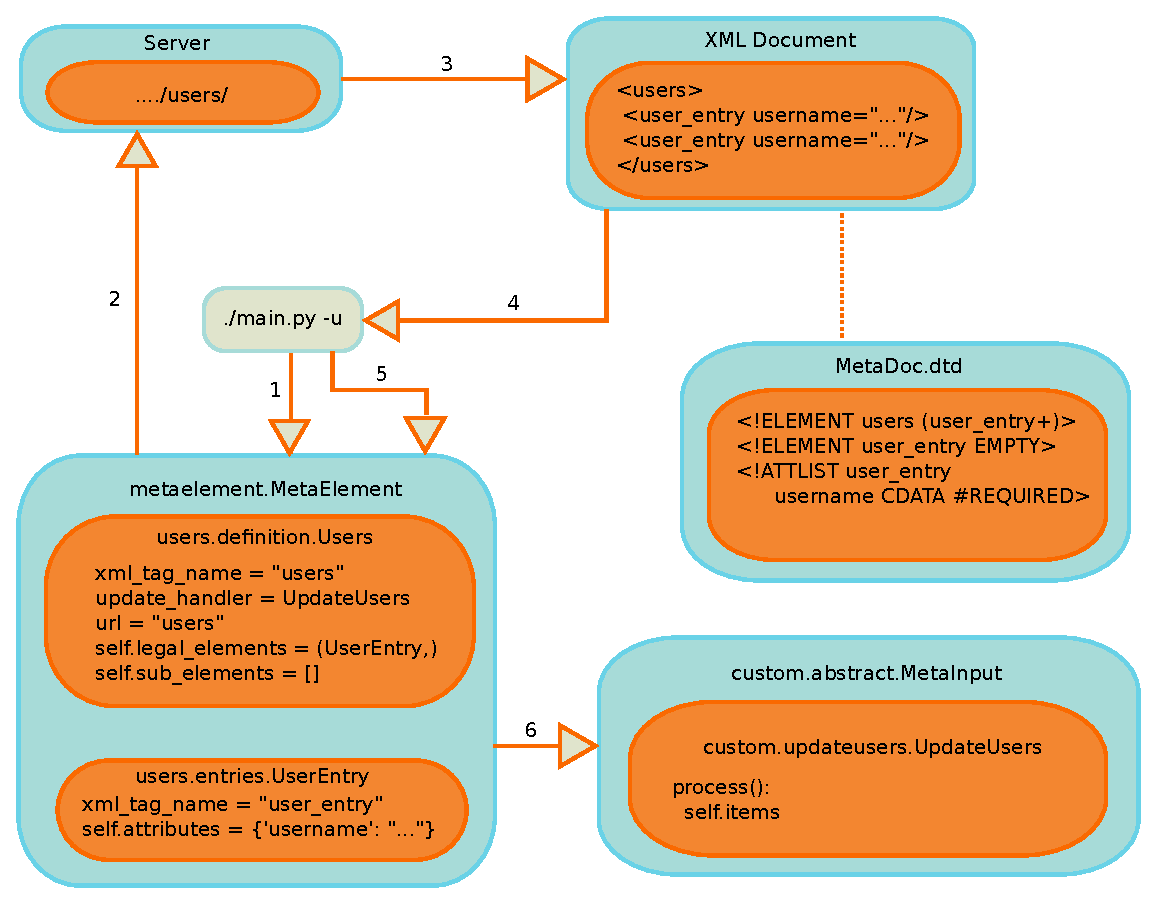
\includegraphics[width=\textwidth]{img/xml_flow}
    \caption{Information flow when requesting user list with MetaDoc}
    \label{fig:information_flow}
\end{figure}

\newpage
\section{Included examples}
\texttt{doc/examples/} includes a set of examples for using MetaDoc. Below is a
list of the included examples and what they do. 

\begin{description}
    \item[cli/event.py] A command line interface for adding events. Should be
    placed inside \texttt{client/} when run. See \texttt{event.py --help} for
    usage.
    \item[custom/updateusers.py]    Custom function for converting recieved
    user data into a passwd/shadow file.
    \item[custom/updateprojects.py] Custom function for converting recieved
    project data to a project user file.
    \item[custom/updateallocations.py]  Custom function for converting recieved
    allocation data into a quota file for projects.
\end{description}

\end{document}
